\chapter{Experiment setup}
\label{chapter:experiment_setup}

In this chapter we describe the data used for experiments, training setup and In this chapter we describe the data, training setup and experiments that were run to answer the questions asked in this thesis.

\section{Questions and constraints}
\label{section:questions_and_constraints}
\todo{Limited resources, reasonable quality is still needed}

Constraints:
\begin{displayquote}
	Translation quality for multi-lingual system is insignificantly worse than for
	mono-lingual one-to-one tranlsation system.

	Maximum possible target languages are combined in one model.
\end{displayquote}

Questions:
\begin{displayquote}
	How \emph{in average} adding one more randomly selected target language
	to the multitarget model affects its En\to{}De performance?

	How is it different if we add a linguistically similar, not randomly selected language?

	How is adding one more language from the same language family or group 
	\emph{in average} affects tranlsation performance for selected language
	pair (e.g. En\to{}De)?
\end{displayquote}



\section{Experiments}
\label{section:experiments}
\subsection{Starting point}
\label{subsection:starting_point}

In \cite{johnson-etal-2017-googles} autors proposed a way to build a multi-lingual
machine tranlsation model without any changes to the \emph{Transformer} architecture.
In fact, the only change should be performed on the input data. To make the \emph{Transformer}
model process multi-lingual data the language tag is added to the source sentence.
For example, the following En\to{}Cz sentence pair:

\begin{displayquote}
Hello world! \to{} Ahoj světe!
\end{displayquote}
is modified to:

\begin{displayquote}
\tagto{cs} Hello world! \to{} Ahoj světe!
\end{displayquote}

With given method it is possible to produce translations in multiple languages using the
same model just by altering the prepended target language tag.
It was also demonstrated that this method slightly improves translation quality for 
low resource languages when compared to monolingual translation model.

In this and the following
(\perscite{arivazhagan-2019-mmnmt-in-the-wild}, \perscite{aharoni-etal-2019-massively})
papers from Google many different cases are tried and described.
However, in each setting there is usually only one model of each kind considered.
For example, when in \parcite{aharoni-etal-2019-massively} authors compare 5-to-5,
25-to-25, 50-to-50, etc. models, there is only one 5-to-5 model, one 25-to-25, etc.


\subsection{Proposed experiments}
\label{subsection:proposed_experiments}

% Given the questions and constraints given in \ref{section:questions_and_constraints},
% the variable object in experiments is the data itself. Due to that, the setup similar
% to \cite{johnson-etal-2017-googles} was chosen. 

\subsubsection*{Monolingual baseline}

Target language tags do not affect \acrshort{bleu}: \perscite{siddhant-2020-x-ling-effect}.
mNMT models en-to-4 and 4-to-en trained;
 1) \tagto{xx} added to the source;
 2) target language encoded separately.
\acrshort{bleu} scores are comparable using both approaches.

\subsubsection*{n-lingual baselines (random)}

Multilingual models with random set of languages.
The purpouse is twofold: 
to show \acrshort{bleu} score decrease with increasing number of target languages and
to serve as a baseline for multitarget models with target languages grouped by
in non-random way, e.g. by language group or linguistic similarity.

\subsubsection*{Group by language group}

If all target languages are from one language group we expect to observe
better translation quality comparing to multilingual baseline results 
with randomly selected target languages.
This is expected due to shared parts of vocabulary (todo: expand with examples)
and linguistic properties (again, expand with examples).
Germanic group: da, de, is, no, nl, sv.
Slavic with cyrillic script: bg, mk, ru, uk.
Slavic: bg, cs, hr, mk, pl, ru, sk, sl, sr, uk

\subsubsection*{Group by linguistic similarity}

From \perscite{siddhant-2020-x-ling-effect} follows that languages' script
and similarly the amount of shared vocabulary is not so important
for XX\to{}En translation direction.
Example with Serbian and Croatian, with the same vocabulary but
in different scripts.





\section{Dataset(s)}
\label{section:datasets}


\subsection{English to 36 languages}
\label{dataset:en-to-36}

To observe effects of linguistic similarity of target languages
it is important to examine enough possible variations of those.
The OPUS dataset (\cite{TIEDEMANN12.463}) is an open and free collection of texts
that covers more than 90 languages with data from several
domains.\footnote{Available at \url{http://opus.nlpl.eu/}} 

For our experiments the source language is English only.

Sampling and splitting of the data is the one used for
ELITR project.\footnote{\url{https://elitr.eu/wp-content/uploads/2019/07/D11.FINAL_.pdf}}
For each of language pairs and each sub-dataset
the data was splitted to training, validation and testing sets.
For each of the two latter sets 2000 random sentences were selected
and the rest of the data remained for the training set.
In cases where the sub-dataset contained less than 16000 sentence pairs
no data went to the validation set.
Later for each language pair there were 1000000 sentence pairs
sampled from all training sub-sets.
Firstly, if available, the sentences were taken from Europarl,
then EUbooks, OpenSubtitles, and then all remaining sub-datasets.
The same procedure was used to sample x000 of validation set sentences
per each language pair.
The test sets were left separate, so that the result on each domain would be observable.

Later an overlap in the source side of different language pairs was found.
Although this would not directly lead to unfair increase of the test score,
such sentence pairs were removed from the training sets.
This filtering decreased the amound of sentence pairs
to 0.85-0.95 millions per language pair.

\begin{figure}[h]
	\centering
	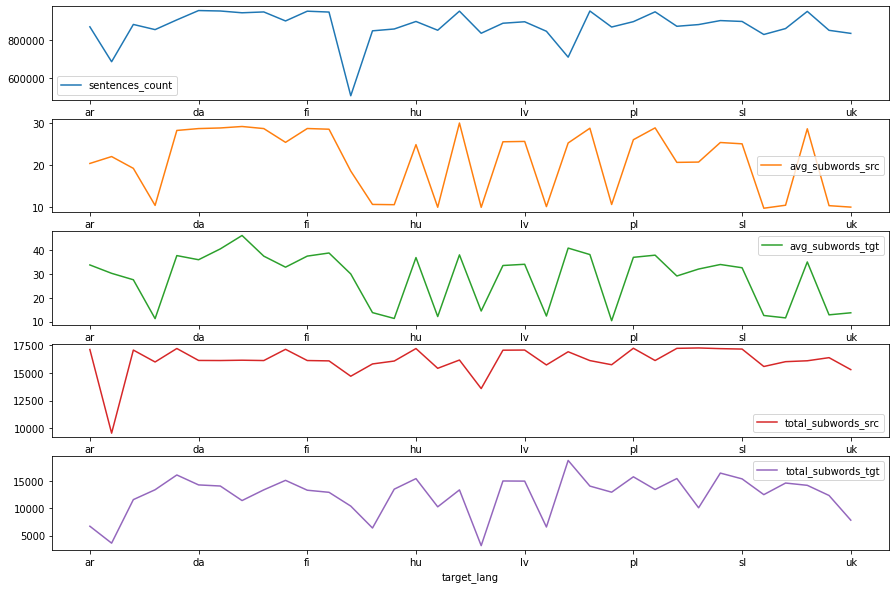
\includegraphics[width=0.9\columnwidth]{../img/train_set_statistics.png}
	\mycaption{Training data language statistics}{
		Languages are on the \emph{X} axis sorted as in appendix.
		From top to bottom:
		total number of sentence pairs in training set per language,
		average amount of subwords per sentence on the source side,
		the same on the target side,
		total amount of unique subwords for this target language on the source side,
		the same on the target side.
	}
	\label{fig:language_statistics}
\end{figure}


To train a model on a specific subset of target languages, only related sentence
pairs are subsampled.
For example, to prepare data for En\to{}$\{$Fr, De$\}$ setup only sentences which source
side starts with tags \tagto{fr} or \tagto{de} are selected to the training set.
Development set is selected in the same way.


\section{Training}

\subsection{Tool kits}

There exists a number of different tools that can be used for training a NMT model.
General purpouse deep learning programming libraries like
Tensorflow\footnote{\url{https://tensorflow.org/}} and
PyTorch\footnote{\url{https://pytorch.org/}} are most popular for deep learning related
research. With their help it is possible to construct any of today's state-of-the-art
NMT models; pre-built and pre-trained models are initially present in such frameworks,
but it is also possible to describe a model from scratch.

Another option is presented by specialized NMT tool kits.
They usually contain efficient and tested implementations of NMT models as well as some of
usefull preprocessing tools.
For the experiments described in \ref{section:experiments} there is a need to train significant
amount of models with the same architecture and settings but different datasets.
Due to that fact, in this work the use of specialized NMT tool kit is more suitable.
Let us consider the foolowing list of broadly used tool kits as for year 2020,
presented in \cite{koehn_2020}:

\begin{itemize}
  \item OpenNMT (based on Torch/pyTorch)\footnote{\url{https://opennmt.net}}
  \item Sockeye (based on MXNet)\footnote{\url{https://github.com/awslabs/sockeye}}
  \item Fairseq (based on pyTorch)\footnote{\url{https://github.com/pytorch/fairseq}}
  \item Marian (stand-alone implementation in C++)\footnote{\url{marian-nmt.github.io}}
  \item Google's Transformer (based on Tensorflow)\footnote{\url{
    https://github.com/tensorflow/models/tree/master/official/transformer}}
  \item Tensor2Tensor (based on Tensorflow) \footnote{\url{
    https://github.com/tensorflow/tensor2tensor}}
\end{itemize}

We chose \textit{MARIAN-NMT} tool kit\footnote{\cite{mariannmt}} as a fast solution
with stable and efficient \textit{Transformer} \cite{vaswani-2017-transformer} implementation,
minimum of third-party dependencies, and ability to train models on multiple GPU units in parallel.


\subsection{Computational cluster}

In the experiments proposed above the expected number of models to be trained is quite big.
First of all, there should be 36 models for \textit{mono-target baseline} for En\to{}36 dataset.
For \textit{multi-target random} experiment the number is much bigger.
For example, let us consider a case with En\to{}3 models - each model translates from English to 
3 target languages. Specifying that each of 36 target languages from En\to{}36 dataset
should appear at least in 3 En\to{}3 models, series of random generation of En\to{}3 setups gave
the smallest amount of such setups equal to 44. For En\to{}5 case with 5 target languages in each
model and with the same restriction of minimum occurance the same procedure gave the
minimum amount of needed models equal to 34.

To be able to train large number of models in a reasonable amount of time we needed to use
computational cluster with GPU cards.
The computational clusters available at the institution are operating under
SGE\footnote{\url{https://arc.liv.ac.uk/trac/SGE}} scheduling software and are equipped with
GPU cards with minimum CUDA \textit{compute capability} 6.1.

Considering data storage quota limitation and high utilization of computational resources by
the cluster's users, the following training pipeline was designed:

\begin{outline}
    \1 Prepare task list
    \1 Iterate over the list working with at most N tasks in parallel
    \1 For each task
        \2 Subsample the dataset taking only those sentence pairs with target languages
	   specified in the task
	\2 Run the training procedure for limited amount of time (e.g. for one hour only)
	   starting with previous checkpoint if it already exists
	\2 Regularly compute metrics on the developement set and report them
	\2 On the event of evaluation on the developenemt set save the best model for each metric
	\2 After time is out the training is stopped and subsampled datasets are removed
    \1 If for next selected task the model is already trained then select next task from the list
    \1 If for next selected task the model is currently being trained then decrease
       the number N of tasks processed in parallel
\end{outline}


\subsection{Inspecting the training process}

As the number of models trained and being trained is growing, monitoring of the training
process becomes more and more complicated. If the experiments are also being run on different
computational clusters it becomes very possible that a parameter mistakenly set up to different
value or a corrupted dataset, or even hardware version may lead to an unexpected difference in results.

To address these and other issues that may occur during the training process we use
Weights$\&$Biases\footnote{\cite{wandb}} experiment tracking tool.
Its main features that are useful in this prospective are following:
\begin{outline}
	\1 Metric visualization
		\2 Training and validation loss curves
		(Figure \ref{fig:single-lang-group-vs-random-dashboard} left subplot)
		\2 Scatter plots (Figures \ref{fig:inspect-convergence}
		and \ref{fig:single-lang-group-vs-random-dashboard} middle subplot)
	\1 Artifact storage
		\2 Model checkpoints storage
			\3 stores 'heavy' model files which cannot be stored
			in \emph{git}
			\3 along with \emph{git} it makes possible to move training
			to the different computational cluster system
		\2 Sample translations of validation set
			\3 helps to observe improvements of translation quality
			in time
			\3 lets verify that model is actually produces meaningfull
			translation
	\1 Customizable reports
	\1 Hardware utilization
\end{outline}

\begin{figure}[h]
	\centering
	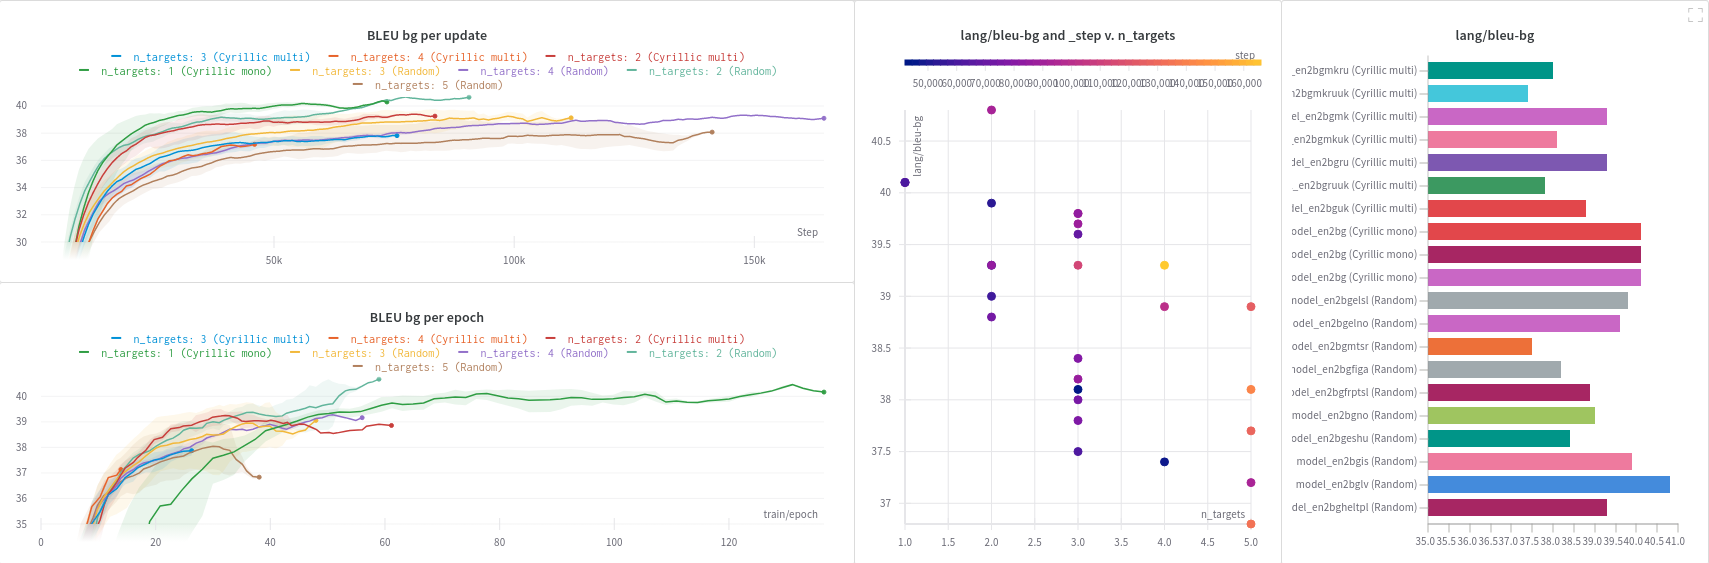
\includegraphics[width=1.0\columnwidth]{../img/slavic_cyrillic_bg.png}
	\mycaption{%
		Single language results visualization: models other target languages are randomly selected
		vs. those selected from similar group of languages
	}{
		\todo{split it in print-friendly way}
		Here is a part of interactive report for 'slavic languages with cyrillic script vs. random'
		experiment. In this specific case models' performace on Bulgarian part of
		validation set is compared.

		\emph{Left}: \acrshort{bleu} score for En\to{}Bg translation direction is monitored with
		training step on \emph{X} axis (top) and training epoch  (bottom).
		Each curve represents mean value (line) and its min/max value
		(range) at the point of time of multiple models' results.
		Models are grouped by number of target languages and experiment subgroup
		(En\to{}Bg, En\to{}Slavic and En\to{}Random).

		\emph{Middle}: Number of targets (axis \emph{X}) vs.
		\acrshort{bleu} on En\to{}Bg validation set (axis \emph{Y}) vs.
		update steps (colos with scale at the top).

		\emph{Right}: Individual models' En\to{}Bg validation \acrshort{bleu} scores.
	}
	\label{fig:single-lang-group-vs-random-dashboard}
\end{figure}


\begin{figure}[h]
	\begin{minipage}{0.8\textwidth}
	\centering
	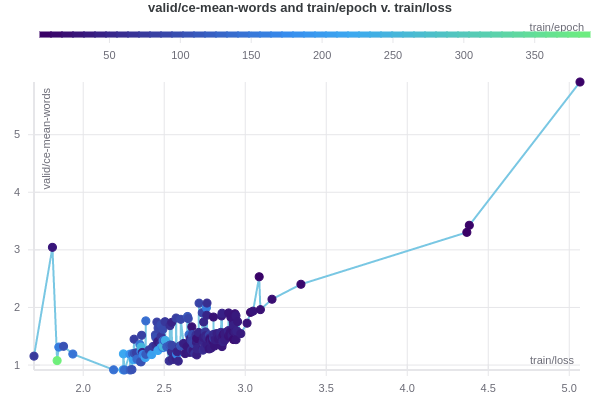
\includegraphics[width=1.0\columnwidth]{../img/inspect_overfit.png}
	\end{minipage}\hfill
	\begin{minipage}{0.8\textwidth}
	\centering
	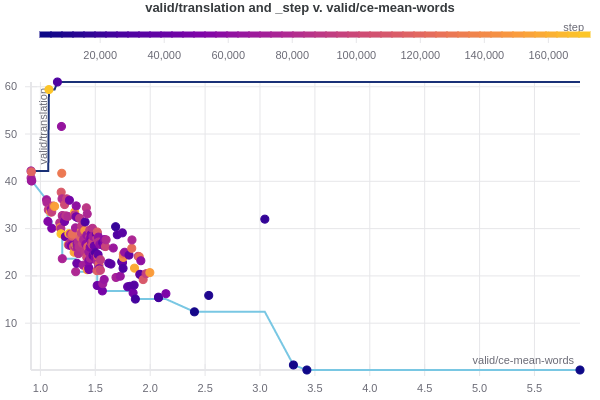
\includegraphics[width=1.0\columnwidth]{../img/inspect-bleu-vs-loss.png}
	\end{minipage}
	\mycaption{%
		Overall model convergence dashboard%
	}{
		On these two interactive graphs each point represents one model.
		Models that are currently training are visualized here together with
		completely converged models and those which training process is currently
		on hold.

		\emph{Left}: axis \emph{X} represents the training loss value,
		axis \emph{Y} represents the value for the same loss function calculated
		on the validation set. The color of each point represents current training
		epoch for the model. Normally for any model the point moves from top right
		part of this graph to the bottom left part, representing both training and
		validation loss being gradually decreased during the training procedure.
		The point that moves to the middle left part of the graph may signalize about
		either \emph{overfitting} of the model on training set, or difference in data
		distribution in training and validation set, or else some mistake in training
		settings.

		\emph{Right}: on this plot loss value on the validation set (axis \emph{X})
		is compared with geometric mean of \acrshort{bleu} scores
		for each of target languages.
		For any model during the training procedure its point usually moves from
		bottom right corner into the cluster of other points.
		Model which point 'arrives' to any other location than the cluster may need
		special attention.
	}
	\label{fig:inspect-convergence}
\end{figure}



\subsection{Model settings}

The initial parameter selection is made with respect to \cite{training-tips}.
First of all, the hyperparameters of MT model are tuned
on couple of language pairs from one dataset.
The parameters leading to the same result in shorter time were preferred.
Then the selected parameters were used on all experimends with the dataset.
